\documentclass[a4paper, 11pt]{article}
\usepackage{amsmath}
\usepackage{graphicx}
\usepackage{geometry}
\usepackage{listings}
\usepackage{xcolor}
\usepackage[colorlinks,linkcolor=red]{hyperref}
\geometry{scale=0.8}
\usepackage[UTF8]{ctex}
\title{	
\normalfont \normalsize
\textsc{School of Data and Computer Science, Sun Yat-sen University} \\ [25pt] %textsc small capital letters
\rule{\textwidth}{0.5pt} \\[0.4cm] % Thin top horizontal rule
\huge  E08 Bayesian Network\\ % The assignment title
\rule{\textwidth}{2pt} \\[0.5cm] % Thick bottom horizontal rule
\author{18340052            何泽}
\date{\normalsize\today}
}

\begin{document}
\maketitle
\tableofcontents
\newpage
\section{Pomegranate Installation}
\textbf{Under Linux:}
\begin{enumerate}
\item Install \texttt{python} first (\textbf{python 2}, not python 3).
\item Run \texttt{sudo apt-get install python-pip} to install \texttt{pip}.
\item Run \texttt{sudo pip install pomegranate} to install \texttt{pomegranate}.
\end{enumerate}
\begin{figure}[h]
  \centering
  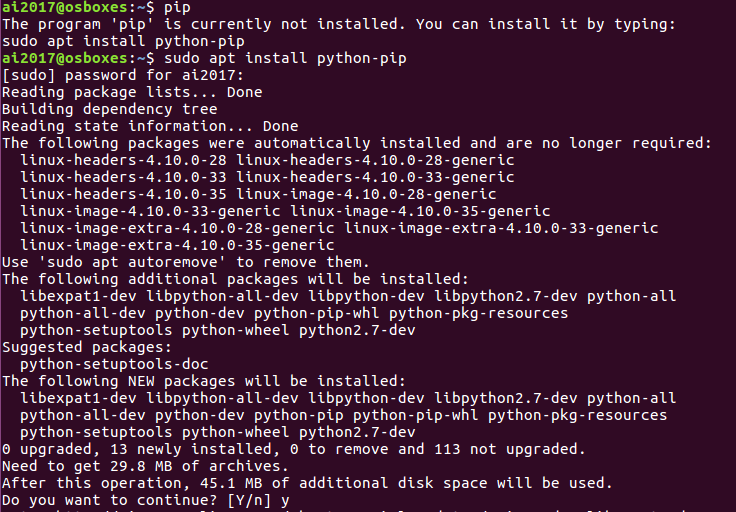
\includegraphics[width=7.5cm]{Pic/install1}
  \qquad
  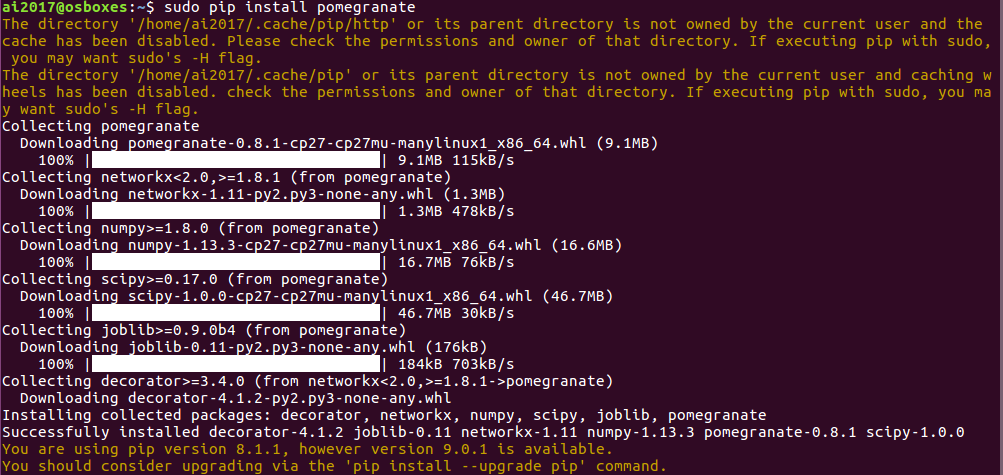
\includegraphics[width=8cm]{Pic/install2}
\end{figure}
\textbf{Under Windows}

You can also run \texttt{pip install pomegranate} if you have installed \texttt{pip}. If you don't know how to install \texttt{pip}, please click \url{https://jingyan.baidu.com/article/e73e26c0d94e0524adb6a7ff.html}.

For more, please click the homepage of Pomegranate - \url{https://github.com/jmschrei/pomegranate} for help. 
\begin{figure}[h]

  
  \centering
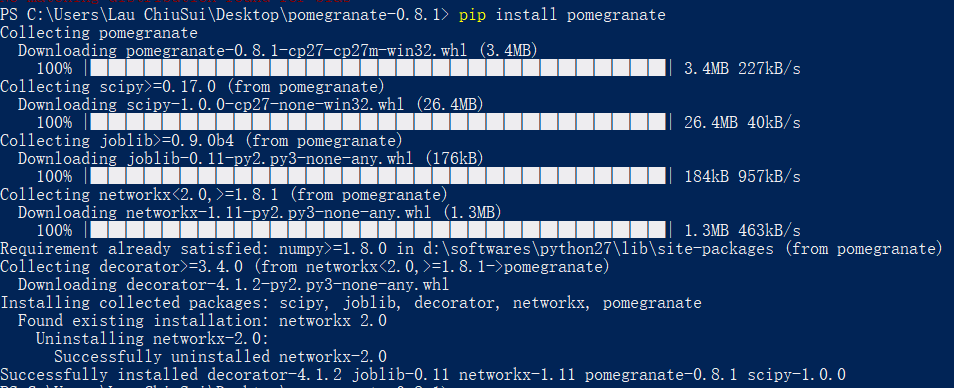
\includegraphics[width=16cm]{Pic/po}
  
\end{figure}

\section{Building Bayesian Network}
\label{sec:build-bayes-netw}
Please refer to \texttt{Tutorial\_4\_Bayesian\_Networks.pdf}. I will explain it in class.

\section{Tasks}
\label{sec:tasks}

\subsection{Burglary}
\label{sec:burglary}
\begin{figure}[h]
  \centering

  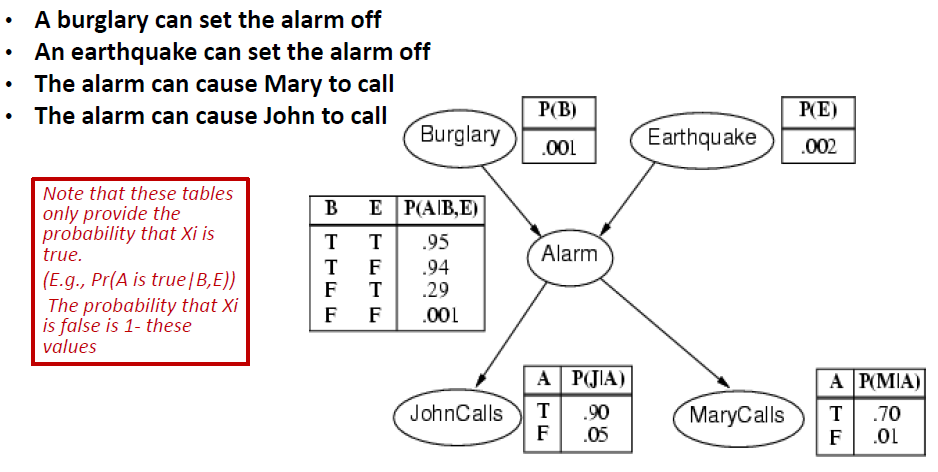
\includegraphics[width=14cm]{Pic/burglary}
\end{figure}
Please code to calculate:
\begin{enumerate}
\item $P(A)$
\item $P(J\overline{M})$
\item $P(A | J\overline{M})$
\item $P(B | A)$
  \item $P(B | J\overline{M})$
  \item  $P(J\overline{M} | \overline{B})$
\end{enumerate}
\begin{figure}[ht]
\centering
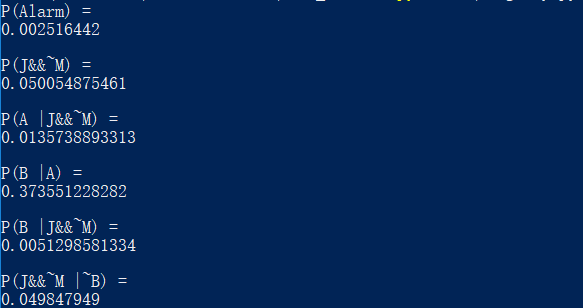
\includegraphics[width=12cm]{Pic/burglar_result}
\end{figure}
\subsection{Diagnosing}
\label{sec:bayesian-networks}
\textbf{Variables and their domais}
\begin{lstlisting}{language=Python}
(1)PatientAge:['0-30','31-65','65+']
(2)CTScanResult:['Ischemic Stroke','Hemmorraghic Stroke']
(3)MRIScanResult: ['Ischemic Stroke','Hemmorraghic Stroke']
(4)StrokeType: ['Ischemic Stroke','Hemmorraghic Stroke', 'Stroke Mimic']
(5)Anticoagulants: ['Used','Not used']
(6)Mortality:['True', 'False']
(7)Disability: ['Negligible', 'Moderate', 'Severe']
\end{lstlisting}
\textbf{CPTs}

\textbf{Note:} [CTScanResult, MRIScanResult,StrokeType] means:

P(StrokeType='...' $|$ CTScanResult='...' $\land$  MRIScanResult='...') 
\begin{lstlisting}{language=Python}
(1)
[PatientAge]

['0-30', 0.10],
['31-65', 0.30],
['65+', 0.60]

(2)
[CTScanResult]

['Ischemic Stroke',0.7],
[ 'Hemmorraghic Stroke',0.3]

(3)
[MRIScanResult]

['Ischemic Stroke',0.7],
[ 'Hemmorraghic Stroke',0.3]

(4)
[Anticoagulants]

[Used',0.5],
['Not used',0.5]

(5)
[CTScanResult, MRIScanResult,StrokeType])

['Ischemic Stroke','Ischemic Stroke','Ischemic Stroke',0.8],
['Ischemic Stroke','Hemmorraghic Stroke','Ischemic Stroke',0.5],  
[ 'Hemmorraghic Stroke','Ischemic Stroke','Ischemic Stroke',0.5],
[ 'Hemmorraghic Stroke','Hemmorraghic Stroke','Ischemic Stroke',0], 

['Ischemic Stroke','Ischemic Stroke','Hemmorraghic Stroke',0],
['Ischemic Stroke','Hemmorraghic Stroke','Hemmorraghic Stroke',0.4], 
[ 'Hemmorraghic Stroke','Ischemic Stroke','Hemmorraghic Stroke',0.4],
[ 'Hemmorraghic Stroke','Hemmorraghic Stroke','Hemmorraghic Stroke',0.9],

['Ischemic Stroke','Ischemic Stroke','Stroke Mimic',0.2],
['Ischemic Stroke','Hemmorraghic Stroke','Stroke Mimic',0.1],    
[ 'Hemmorraghic Stroke','Ischemic Stroke','Stroke Mimic',0.1],
[ 'Hemmorraghic Stroke','Hemmorraghic Stroke','Stroke Mimic',0.1],

(6) 
[StrokeType, Anticoagulants, Mortality]

['Ischemic Stroke', 'Used', 'False',0.28],
['Hemmorraghic Stroke', 'Used', 'False',0.99],
['Stroke Mimic', 'Used', 'False',0.1],
['Ischemic Stroke','Not used', 'False',0.56],
['Hemmorraghic Stroke', 'Not used', 'False',0.58],
['Stroke Mimic', 'Not used', 'False',0.05],

['Ischemic Stroke',  'Used' ,'True',0.72],
['Hemmorraghic Stroke', 'Used', 'True',0.01],
['Stroke Mimic', 'Used', 'True',0.9],
['Ischemic Stroke',  'Not used' ,'True',0.44],
['Hemmorraghic Stroke', 'Not used', 'True',0.42 ],
['Stroke Mimic', 'Not used', 'True',0.95]

(7)
[StrokeType, PatientAge, Disability]

['Ischemic Stroke',   '0-30','Negligible', 0.80],
['Hemmorraghic Stroke', '0-30','Negligible', 0.70],
['Stroke Mimic',        '0-30', 'Negligible',0.9],
['Ischemic Stroke',     '31-65','Negligible', 0.60],
['Hemmorraghic Stroke', '31-65','Negligible', 0.50],
['Stroke Mimic',        '31-65', 'Negligible',0.4],
['Ischemic Stroke',     '65+'  , 'Negligible',0.30],
['Hemmorraghic Stroke', '65+'  , 'Negligible',0.20],
['Stroke Mimic',        '65+'  , 'Negligible',0.1],

['Ischemic Stroke',     '0-30' ,'Moderate',0.1],
['Hemmorraghic Stroke', '0-30' ,'Moderate',0.2],
['Stroke Mimic',        '0-30' ,'Moderate',0.05],
['Ischemic Stroke',     '31-65','Moderate',0.3],
['Hemmorraghic Stroke', '31-65','Moderate',0.4],
['Stroke Mimic',        '31-65','Moderate',0.3],
['Ischemic Stroke',     '65+'  ,'Moderate',0.4],
['Hemmorraghic Stroke', '65+'  ,'Moderate',0.2],
['Stroke Mimic',        '65+'  ,'Moderate',0.1],

['Ischemic Stroke',     '0-30' ,'Severe',0.1],
['Hemmorraghic Stroke', '0-30' ,'Severe',0.1],
['Stroke Mimic',        '0-30' ,'Severe',0.05],
['Ischemic Stroke',     '31-65','Severe',0.1],
['Hemmorraghic Stroke', '31-65','Severe',0.1],
['Stroke Mimic',        '31-65','Severe',0.3],
['Ischemic Stroke',     '65+'  ,'Severe',0.3],
['Hemmorraghic Stroke', '65+'  ,'Severe',0.6],
['Stroke Mimic',        '65+'  ,'Severe',0.8]
\end{lstlisting}
\textbf{Calculation}

Please code to calculate the following probability value:

p1 = P(Mortality='True' $|$ PatientAge='31-65' $\land$ CTScanResult='Ischemic Stroke')

p2 = P(Disability='Moderate' $|$ PatientAge='65+' $\land$  MRIScanResult='Hemmorraghic Stroke')

p3 = P(StrokeType='Stroke Mimic' $|$ PatientAge='65+' $\land$ CTScanResult='Hemmorraghic Stroke' $\land$ MRIScanResult='Ischemic Stroke')

p4 = P(Anticoagulants='Not used' $|$ PatientAge='0-30')

\begin{figure}[ht]
\centering
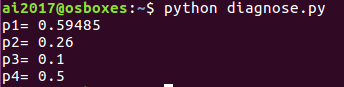
\includegraphics[width=12cm]{Pic/diagnose_result}
\end{figure}

Please solve the 2 tasks and hand in a file named \textsf{E08\_YourNumber.pdf}, and send it to \textsf{ai\_2020@foxmail.com}


\section{Codes and Results}
\subsection{Burglary}
Code:
\lstset{
	columns=fixed,       
	numbers=left,                                        % 在左侧显示行号
	frame=shadowbox,                                          % 不显示背景边框
	backgroundcolor=\color[RGB]{245,245,244},            % 设定背景颜色
	keywordstyle=\color[RGB]{0,92,230},                 % 设定关键字颜色
	numberstyle=\footnotesize\color{darkgray},           % 设定行号格式
	commentstyle=\it\color[RGB]{0,96,96},                % 设置代码注释的格式
	stringstyle=\rmfamily\slshape\color[RGB]{230,92,0},   % 设置字符串格式
	showstringspaces=false,                              % 不显示字符串中的空格
	breaklines,
	language=Python,      
}
\begin{lstlisting}
from pomegranate import *

Burglary = DiscreteDistribution( {'T':0.001, 'F':0.999} )
Earthquake = DiscreteDistribution( {'T':0.002, 'F':0.998} )
Alarm = ConditionalProbabilityTable(
    [
        ['T','T','T',0.95],
        ['T','F','T',0.94],
        ['F','T','T',0.29],
        ['F','F','T',0.001],
        ['T','T','F',0.05],
        ['T','F','F',0.06],
        ['F','T','F',0.71],
        ['F','F','F',0.999],
    ], 
    [Burglary, Earthquake]
)

JohnCalls = ConditionalProbabilityTable(
    [
        ['T','T',0.90],
        ['F','T',0.05],
        ['T','F',0.10],
        ['F','F',0.95],
    ], 
    [Alarm]
)
    
MaryCalls = ConditionalProbabilityTable(
    [
        ['T','T',0.70],
        ['F','T',0.01],
        ['T','F',0.30],
        ['F','F',0.99],
    ], 
    [Alarm]
)

s1 = State(Burglary, name="Burglary")
s2 = State(Earthquake, name="Earthquake")
s3 = State(Alarm, name="Alarm")
s4 = State(JohnCalls, name="JohnCalls")
s5 = State(MaryCalls, name="MaryCalls")

model = BayesianNetwork("Burglary")
model.add_states(s1,s2,s3,s4,s5)
model.add_transition(s1,s3)
model.add_transition(s2,s3)
model.add_transition(s3,s4)
model.add_transition(s3,s5)
model.bake()
marginals = model.predict_proba({})

print("P(Alarm) = {}".format(marginals[2].parameters[0]["T"]))

p2 = model.predict_proba({'MaryCalls':'F'})[3].parameters[0]["T"] * marginals[4].parameters[0]["F"]
print("P(J && ~M) = {}".format(p2))

print("P(A | J && ~M) = {}".format(model.predict_proba({'JohnCalls':'T','MaryCalls':'F'})[2].parameters[0]["T"]))

print("P(B | A) = {}".format(model.predict_proba({'Alarm':'T'})[0].parameters[0]["T"]))

p5 = model.predict_proba({'JohnCalls':'T','MaryCalls':'F'})[0].parameters[0]["T"]
print("P(B | J && ~M) = {}".format(p5))

print("P(J && ~M | ~B) = {}".format((1-p5) * p2 / marginals[0].parameters[0]["F"]))
\end{lstlisting}
Result:
\begin{figure}[ht]
  \centering
  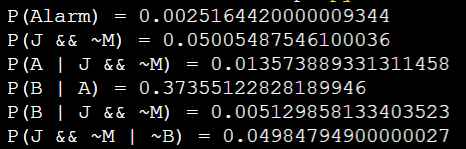
\includegraphics[width=0.9\textwidth]{Pic/1}
  \qquad
\end{figure}

\subsection{Diagnosing}
Code:
\lstset{
	columns=fixed,       
	numbers=left,                                        % 在左侧显示行号
	frame=shadowbox,                                          % 不显示背景边框
	backgroundcolor=\color[RGB]{245,245,244},            % 设定背景颜色
	keywordstyle=\color[RGB]{0,92,230},                 % 设定关键字颜色
	numberstyle=\footnotesize\color{darkgray},           % 设定行号格式
	commentstyle=\it\color[RGB]{0,96,96},                % 设置代码注释的格式
	stringstyle=\rmfamily\slshape\color[RGB]{230,92,0},   % 设置字符串格式
	showstringspaces=false,                              % 不显示字符串中的空格
	breaklines,
	language=Python,      
}
\begin{lstlisting}
from pomegranate import *

PatientAge = DiscreteDistribution({'A': 0.10,'B': 0.30,'C': 0.60})

CTScanResult = DiscreteDistribution({'IS': 0.7,'HS': 0.3})

MRIScanResult = DiscreteDistribution({'IS': 0.7,'HS': 0.3})

Anticoagulants = DiscreteDistribution({'T': 0.5,'F': 0.5})

StrokeType = ConditionalProbabilityTable(
    [
        ['IS', 'IS', 'IS', 0.8],
        ['IS', 'HS', 'IS', 0.5],
        ['HS', 'IS', 'IS', 0.5],
        ['HS', 'HS', 'IS', 0.0],

        ['IS', 'IS', 'HS', 0.0],
        ['IS', 'HS', 'HS', 0.4],
        ['HS', 'IS', 'HS', 0.4],
        ['HS', 'HS', 'HS', 0.9],

        ['IS', 'IS', 'SM', 0.2],
        ['IS', 'HS', 'SM', 0.1],
        ['HS', 'IS', 'SM', 0.1],
        ['HS', 'HS', 'SM', 0.1],
    ],
    [CTScanResult, MRIScanResult]
)

Mortality = ConditionalProbabilityTable(
    [
        ['IS', 'T', 'F', 0.28],
        ['HS', 'T', 'F', 0.99],
        ['SM', 'T', 'F', 0.10],
        ['IS', 'F', 'F', 0.56],
        ['HS', 'F', 'F', 0.58],
        ['SM', 'F', 'F', 0.05],
        ['IS', 'T', 'T', 0.72],
        ['HS', 'T', 'T', 0.01],
        ['SM', 'T', 'T', 0.90],
        ['IS', 'F', 'T', 0.44],
        ['HS', 'F', 'T', 0.42],
        ['SM', 'F', 'T', 0.95],
    ],
    [StrokeType, Anticoagulants]
)

Disability = ConditionalProbabilityTable(
    [
        ['IS', 'A', 'N', 0.80],
        ['HS', 'A', 'N', 0.70],
        ['SM', 'A', 'N', 0.90],
        ['IS', 'B', 'N', 0.60],
        ['HS', 'B', 'N', 0.50],
        ['SM', 'B', 'N', 0.40],
        ['IS', 'C', 'N', 0.30],
        ['HS', 'C', 'N', 0.20],
        ['SM', 'C', 'N', 0.10],

        ['IS', 'A', 'M', 0.10],
        ['HS', 'A', 'M', 0.20],
        ['SM', 'A', 'M', 0.05],
        ['IS', 'B', 'M', 0.30],
        ['HS', 'B', 'M', 0.40],
        ['SM', 'B', 'M', 0.30],
        ['IS', 'C', 'M', 0.40],
        ['HS', 'C', 'M', 0.20],
        ['SM', 'C', 'M', 0.10],

        ['IS', 'A', 'S', 0.10],
        ['HS', 'A', 'S', 0.10],
        ['SM', 'A', 'S', 0.05],
        ['IS', 'B', 'S', 0.10],
        ['HS', 'B', 'S', 0.10],
        ['SM', 'B', 'S', 0.30],
        ['IS', 'C', 'S', 0.30],
        ['HS', 'C', 'S', 0.60],
        ['SM', 'C', 'S', 0.80],
    ],
    [StrokeType, PatientAge]
)

s1 = Node(PatientAge, name="PatientAge")
s2 = Node(CTScanResult, name="CTScanResult")
s3 = Node(MRIScanResult, name="MRIScanResult")
s4 = Node(Anticoagulants, name="Anticoagulants")
s5 = Node(StrokeType, name="StrokeType")
s6 = Node(Mortality, name="Mortality")
s7 = Node(Disability, name="Disability")

model = BayesianNetwork("Diagnosing Problem")
model.add_states(s1, s2, s3, s4, s5, s6, s7)
model.add_edge(s2, s5)
model.add_edge(s3, s5)
model.add_edge(s5, s6)
model.add_edge(s4, s6)
model.add_edge(s5, s7)
model.add_edge(s1, s7)
model.bake()

print('p1= ', model.predict_proba({'PatientAge': 'B', 'CTScanResult': 'IS'})[5].parameters[0]['T'])

print('p2= ', model.predict_proba({'PatientAge': 'C', 'MRIScanResult': 'HS'})[6].parameters[0]['M'])

print('p3= ', model.predict_proba({'PatientAge': 'C', 'CTScanResult': 'HS', 'MRIScanResult': 'IS'})[4].parameters[0]['SM'])

print('p4= ', model.predict_proba({'PatientAge': 'A'})[3].parameters[0]['F'])
\end{lstlisting}
Result:
\begin{figure}[ht]
  \centering
  
\includegraphics[width=0.6\textwidth]{Pic/2}
  \qquad
\end{figure}
%\clearpage
%\bibliography{E:/Papers/LiuLab}
%\bibliographystyle{apalike}
\end{document} 
%%% Local Variables:
%%% mode: latex
%%% TeX-master: t
%%% End:
